\documentclass[12pt]{article}
\usepackage[left=1in, right=1in, top=1in, bottom=1in]{geometry}
\usepackage{graphicx}
\usepackage{url}
\usepackage{cite}
\usepackage{float}
\usepackage{caption}
\usepackage{subcaption}
\usepackage{hyperref}
\hypersetup{
    colorlinks,
    citecolor=black,
    filecolor=black,
    linkcolor=black,
    urlcolor=black
}

\renewcommand{\familydefault}{\sfdefault}


\begin{document}
\begin{titlepage}
    \begin{center}
        \LARGE
        \textbf{ELE 401 - GRADUATION PROJECT I}

        \Large
        \textbf{FIRST INTERIM REPORT}

        \vspace{70pt}

        \textit{
            Hacettepe University \\
            Department of Electrical and Electronics Engineering
        }
    \end{center}
    
    \vspace{90pt}

    \large

    \textbf{Project Title:} Sensor Fusion in the Cloud \\

    \textbf{Project Group Members:} Ertuğrul Tiyek, Ahmet Yusuf Şirin

    \vspace{30pt}

    \textbf{Project Supervisor:} Asst. Prof. Dr. İsmail Uyanık \\

    \textbf{Submission Date:} 05.11.2022

    \vspace{\fill}

    \begin{center}
        \textit{FALL 2022-2023}
    \end{center}
\end{titlepage}

\clearpage

\tableofcontents
\listoffigures
\listoftables

\clearpage

\section{INTRODUCTION}

One of the most important aim of the modern technology is the sensing the environment. Living beings have sense organs to know the environment. They have brains to make fusion the sensor data and augment the environmental information taken from sense organs. For example, human standing in balance, we can say that they use the data coming from their eyes and ears together.

People are studying to make this sensing and augmenting artificially, too. They use computers to achieve this. But computers cannot sense the environment directly. They need some devices called sensors. There are all kinds of sensors to measure different environmental quantities. For same quantity, there are different sensors using different technologies, have different precision and accuracy levels. Each sensor has its advantages and disadvantages. Even sensors that are serving a different purpose can help to augment same information other than their main. This is known as "sensor fusion"~\cite{enwiki:1115352853}. Just like humans, robots are use camera and inertial sensors to stand in balance. 

In our project, sensor fusion handles extracting depth information. Sensor fusion can be implemented using specific algorithms like EKF, CNN etc. according to quantity that will be calculated, number and types of sensors used, accuracy and performance needed. We are planning to develop a sensor fusion algorithm with the help of living organisms. As we mentioned before, living beings perform sensor fusion perfectly. We will be examining the zebra fish and how it processes data of its sense organs to produce depth information. Then we will try to develop similar algorithm or improve our algorithm with data taken from zebra fish. 

Depth information can be used for many applications like automatic driven vehicles, UAVs, Augmented Reality devices and 3D modeling of areas. Our concept in this project will be autonomous controlled SLAM Robot. Simultaneous localization and mapping (SLAM) is the computational problem of constructing or updating a map of an unknown environment while simultaneously keeping track of an agent's location within it~\cite{enwiki:1120084976}. We use a robot to move the system. 

Another concept we aim to use is cloud computing. Mobile computing devices may not match the performance requirements in some cases. To achieve more accurate depth information, complex control algorithms or neural networks will be used in our project which needs high computing power. As an alternative to the mobile computing devices, we may use cloud computing.  

\section{PROJECT DESCRIPTION}

This project aims to construct an unmanned ground vehicle that senses the environment and decides its movements. As mentioned in the "Introduction" section, the sensor fusion and mapping algorithms take a lot of space in this project. In addition to that, there are other parts that need to be implemented like robot controls, data acquisition from sensors and cameras, decision making algorithms etc. 

    \subsubsection*{A. Hardware Architecture of the Project}

    The hardware component choices are explained with consideration of advantages and disadvantages in the section 3.2 Design Constraints. Here we have our main components and specifications of them: 

    \begin{enumerate}
        \item \textbf{Robot – Unitree Go1 Edu} \\
        This robot is a ready-to-go quadruped robot with built-in 5 Sets of Fish-eye Stereo Depth Cameras, Ai Post-processing, 3 Sets of Hypersonic Sensors. There are three Nvidia Jetson Nano, one Raspberry Pi 4, one STM32 Microcontroller devices inside of the Unitree Go1 Edu. These devices located in the robot to perform certain tasks. STM32 Microcontroller drives joint motors of the robot. Raspberry Pi 4 is used for both communicate with user and send commands to STM32. Two of Nvidia Jetson Nano 4GB kits and one Nvidia Jetson Nano 2 GB development kit are used for getting data from camera and sensors, processing raw data to extract dept information of stereo cameras.

        \begin{figure}[H]
            \centering
            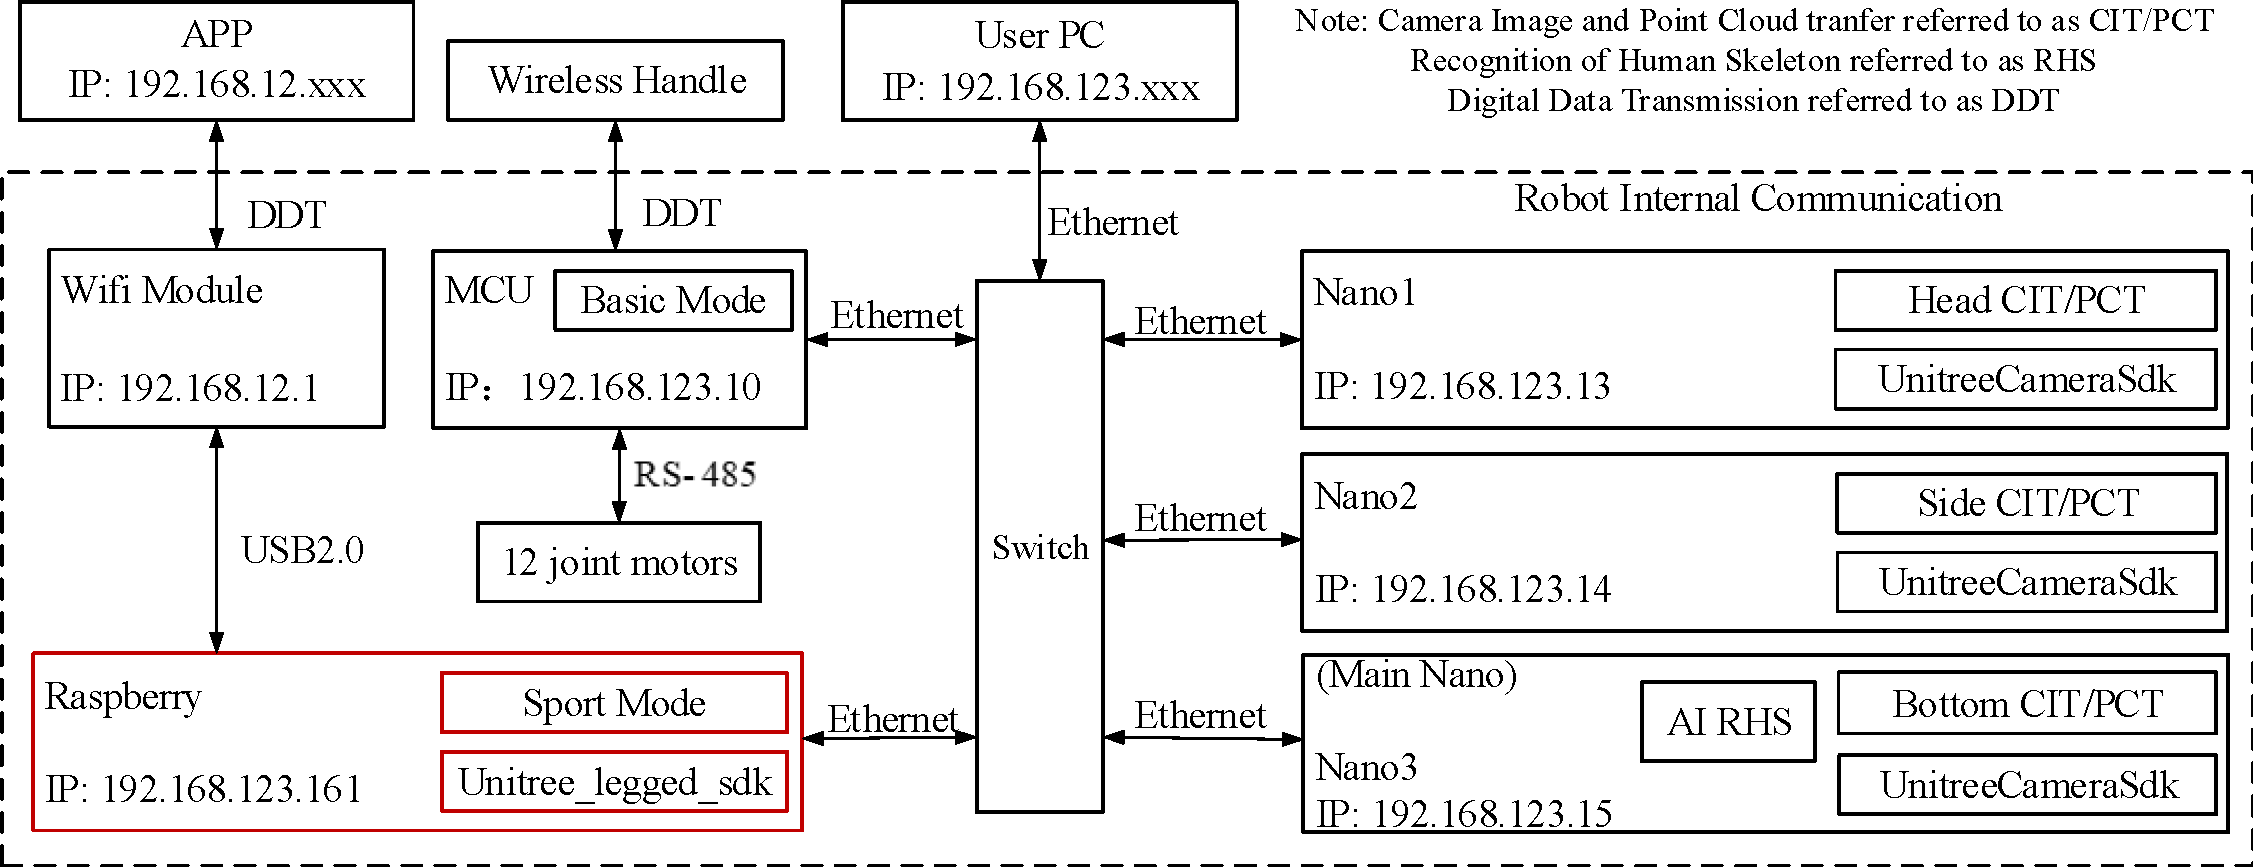
\includegraphics[width=0.9\textwidth]{Go1CommFram_E.png}    
            \caption{Infrastructure of the Unitree Go1 Robot}
        \end{figure}

        The manufacturer provides two Software Development Kits. "unitree\_legged\_sdk” for Controlling the robot, “unitree\_camera\_sdk” for getting camera data and calculating depth information. 

        \item \textbf{Stereo Cameras – Unitree Camera } \\
        There are 5 sets of fish-eye stereo depth cameras located on different important locations of the robot. The known features are:

        \begin{itemize}
            \item Lens Angle $\approx$ 150x170° 
            \item HD (1280x720) , 30fps video streaming 
            \item Raw Frame 
            \item Rectangular Frame 
            \item Depth Frame 
            \item Point Cloud Image 
            \item Provided SDK 
        \end{itemize}
        
        \item \textbf{3D LIDAR – Velodyne 80-VLP-16-A~\cite{VelodyneLiDAR}} \\
        The VLP-16 has a range of 100m, and the sensor's low power consumption (~8W), light weight (830 grams), compact footprint (~Ø103mm x 72mm), and dual return capability make it ideal for UAVs and other mobile applications. 

        Velodyne’s LiDAR Puck supports 16 channels, ~300,000 points/sec, a 360° horizontal field of view and a 30° vertical field of view, with +/- 15° up and down. The Velodyne LiDAR Puck does not have visible rotating parts, making it highly resilient in challenging environments (Rated IP67). 

        Automotive Mapping UAV Security Robotics Automation 

        The module provides up to 0.3 million points/second over 100Mbps ethernet cable and UDP interface. UDP packages contain distances, calibrated reflectivity information, rotation angles, synchronized time stamps (microseconds resolution). 

        \item \textbf{Computation Unit – Nvidia Jetson Nano 4GB} \\
        Unitree Go1 Edu has three Nvidia Jetson Nano Development kits inside it to perform tasks like point cloud, human skeleton tracking etc. We don’t use most of the features robot has, so we decided on using one of the Nvidia Jetson Nano 4GB models in the robot with reducing its 
        workload. 

        Here is some specifications of Nvidia Jetson Nano 4GB~\cite{JatsonNano}: 
        
        \begin{itemize}
            \item GPU		:	128-core Maxwell 
            \item CPU		:	Quad-core ARM A57 @ 1.43 GHz 
            \item Memory	:	4 GB 64-bit LPDDR4 25.6 GB/s 
            \item Storage	:	microSD (not included) 
            \item Camera	:	2x MIPI CSI-2 DPHY lanes 
            \item Connectivity	:	Gigabit Ethernet, M.2 Key E 
            \item Display	:	HDMI and display port 
            \item USB		:	4x USB 3.0, USB 2.0 Micro-B 
            \item Others		:	GPIO, I2C, I2S, SPI, UART 
        \end{itemize}

        As mentioned before, one of the aims of this project is performing heavy computation on cloud. The point of implementing the algorithm on a mobile platform is to keep things simple in the first step. That provides us both simple implementation and ability to make a comparison between mobile computing and cloud computing in terms of performance, accuracy and cost. 

    \end{enumerate}

    \subsubsection*{B. Software Architecture of the Project}

    Laying on the keep it simple stupid (KISS) principle, we separate our project into smaller and independent parts of development.  

    \begin{enumerate}
        \item \textbf{Controlling the Robot Movement and Getting Sensor Data Using Software} \\
        There is a SDK provided by Unitree to control the robot with software called unitree\_legged\_sdk. We used the python programming language with unitree\_legged\_sdk. The details about choice of programming language are explained in the section 3.2 design constraints. 

        Connection between robot and controller computer established via UDP protocol. There are two options that can provide UDP connection. One is the ethernet port of switch that connects all devices in the robot and the other is Wi-Fi access point that connected to the Raspberry Pi 4 in the robot. All devices are using a network mask 255.255.255.0, so it is important to use a static IP on the user computer. 

        \begin{figure}[H]
            \centering
            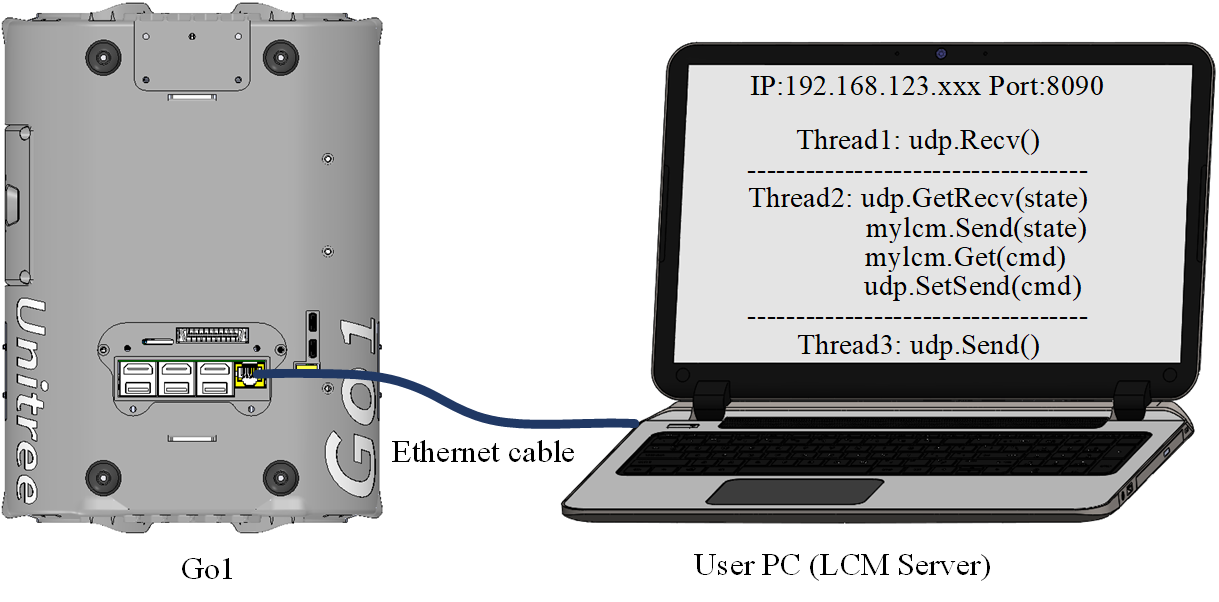
\includegraphics[width=0.8\textwidth]{UserRobotConnection.png}
            \caption{User Robot Connection: Network Mask Settings}
        \end{figure}

        \begin{figure}[H]
            \centering
            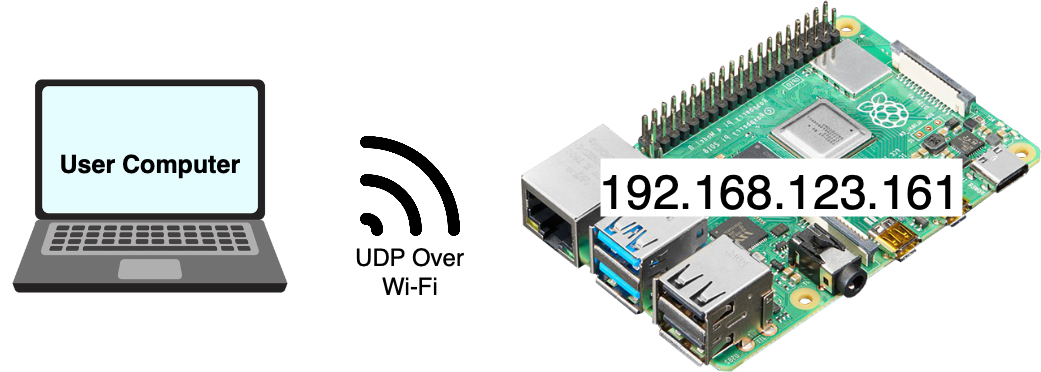
\includegraphics[width=0.8\textwidth]{UserRPiConn.png}
            \caption{User Robot Connection: IP of Raspberry Pi}
        \end{figure}

        Unitree\_legged\_sdk allows both low-level and high-level controls. Low-level control allows user to adjust each joint manually. High-level control provides user to control robot with high-level commands like walk, turn, jump etc. We will be using high-level control for this project. 

        SDK has udp class that provides us an object constructs a UDP connection with Raspberry Pi of Robot. UDP object has functions to receive, send, decode and encode udp packages. 

        Another class included in the SDK is HighState. HighState objects store state information of the robot. It is updated using udp.receive(HighState) function. HighState objects includes IMU measurement information, odometer information, 2D speed information, yaw speed information, position information, body height information etc. 

        To send the commands to the robot, there is a class called CMD in the SDK. CMD object is a command package that tell the robot what to do. CMD package consists of command mode, velocity, yaw speed, target position, required body height variables. Then udp.SetSend(cmd) redyes the cmd object  with encoding it to be sent. Finally the udp object sends the command to the Raspberry Pi using udp.send(). 

        Raspberry Pi 4 also uses unitree\_legged\_sdk to receive commands from and send state information to the user computer. It also communicates with the STM32 Microcontroller which controls all joint motors of the robot. 

        \item \textbf{Getting RGB and Depth Frames from Stereo Cameras (unitree\_camera\_sdk)} \\
        As mentioned before, there are 5 sets of fish-eye stereo depth camera units to both provide an RGB frame and depth frame around the robot.  

        \begin{figure}[H]
            \centering
            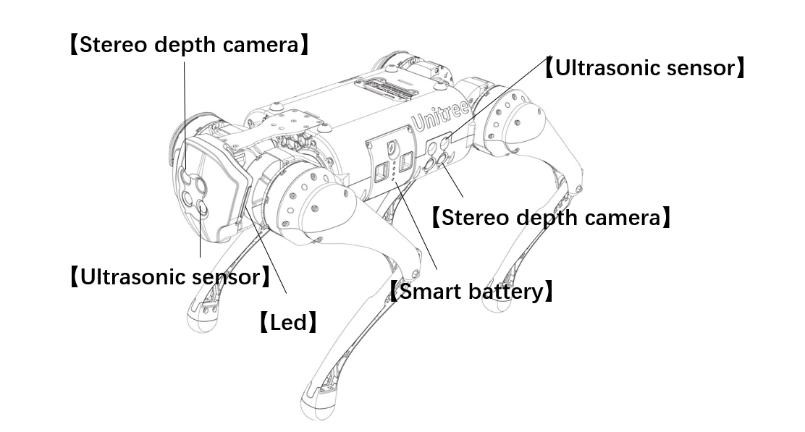
\includegraphics[width=0.8\textwidth]{RobotComponentLocations.jpeg}
            \caption{Legged Robot Sensors and Other Components}
        \end{figure}

        \begin{figure}[H]
            \centering
            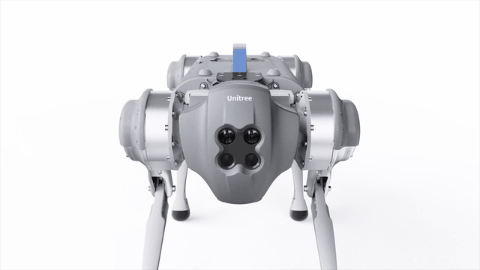
\includegraphics[width=0.8\textwidth]{RobotFront.png}
            \caption{Legged Robot Head Supersensory}
        \end{figure}

        Unitree provides unitree\_camera\_sdk to access camera data of the robot. The SDK allows getting raw frames, rectangular frames, depth frames and point cloud frames. 

        SDK is based on GStreamer framework and works on Nvidia Jetson Nano devices. GStreamer is a library for constructing graphs of media-handling components. Applications can take advantage of advances in codec and filter technology transparently. Developers can add new codecs and filters by writing a simple plugin with a clean, gener~\cite{gstreamer}. GStreamer creates a media pipeline that allows developers to implement their applications simple and modular. 

        unitree\_camera\_sdk creates a pipeline on GStreamer and a virtual video device for each camera connected to the Jetson Nano. Developer can easily read camera information, raw frames, rectangular frames, depth frames and point cloud frames using SDK in their apps. 

        \begin{figure}[H]
            \centering
            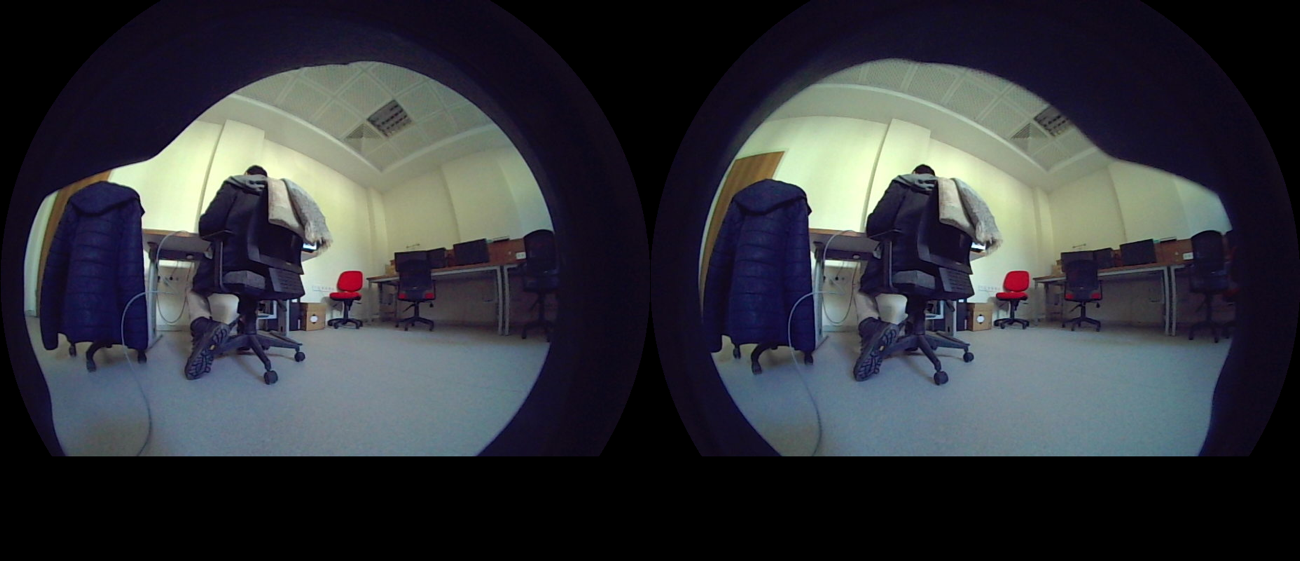
\includegraphics[width=\textwidth]{RawStereo.png}
            \caption{Raw Frame}
        \end{figure}

        \begin{figure}[H]
            \centering
            \begin{subfigure}[b]{0.4\textwidth}
                \centering
                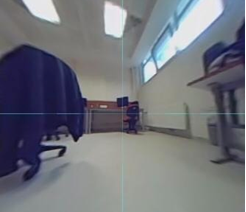
\includegraphics[width=\textwidth]{StereoRectFrame.png}
                \caption{Rectangular Frame}
            \end{subfigure}
            \hfill
            \begin{subfigure}[b]{0.4\textwidth}
                \centering
                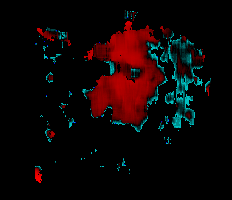
\includegraphics[width=\textwidth]{StereoDeptFrame.png}
                \caption{Depth Frame}
            \end{subfigure}
            \caption{Worked Frames}
        \end{figure}

        Robot has some built in features like human skeleton tracking that uses cameras automatically. There are some services implemented to run these applications automatically while system is starting up. Developer should be whether kill these processes after startup or edit the services not to run processes that uses cameras. 

        Dept information is calculated from stereo camera using stereo vision algorithms. First step is matching each pixel of left frame with corresponding pixel in right frame. This step includes computer vision algorithms like Sum of Squared Differences (SSD) and Sum of Absolute Differences (SAD). 

        \begin{figure}[H]
            \centering
            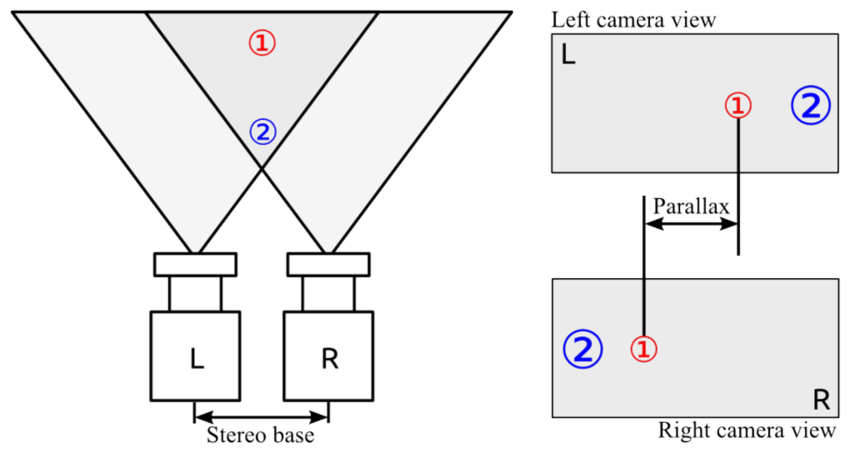
\includegraphics[width=0.8\textwidth]{SSDSAD.png}
            \caption{Sum of Squared Differences (SSD) and Sum of Absolute Differences (SAD)}
        \end{figure}

        After every point matched, distance of every point can be calculated using basic geometric calculations like Thales Theorem. 

        \begin{figure}[H]
            \centering
            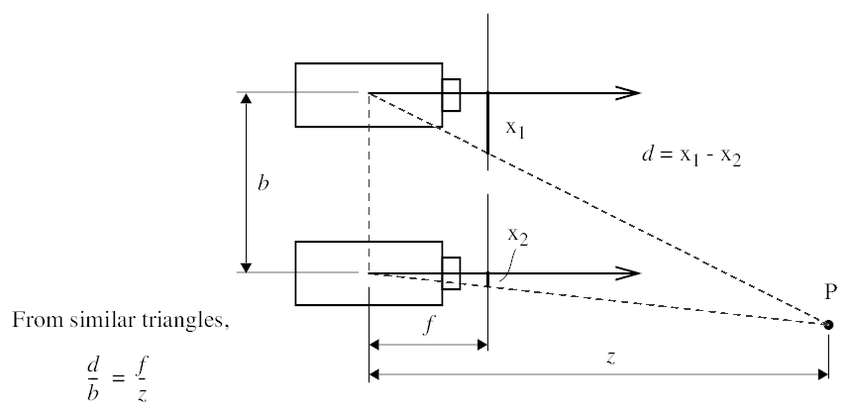
\includegraphics[width=0.8\textwidth]{Thales.png}
            \caption{Thales Theorem}
        \end{figure}

        Stereo cameras provide three dimensional images without using moving parts and high costs. But they have disadvantages as they have advantages. Each camera has lenses to converge and diverge the light coming from different angles and make them fall onto the sensor. That means each camera has a visual angle. Other than that visual angle cannot enter the frame. As we think of the closest points of the baseline of the stereo camera that enters visual angle, it is hard to both match these points in both frames and calculate their distances from camera. Figure shows disparity with respect to distance of the point from baseline of the stereo camera. 

        \begin{figure}[H]
            \centering
            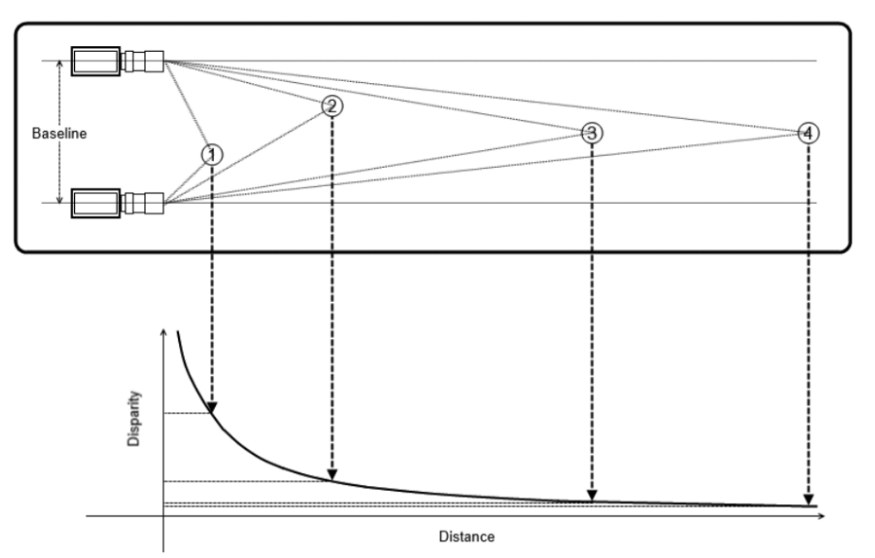
\includegraphics[width=0.6\textwidth]{DisparityOnStereo.png}
            \caption{Disparity with respect to Distance}
        \end{figure}        

        \item \textbf{Developing Sensor Fusion Algorithm for 3D LIDAR and Stereo Cameras}
        \item \textbf{Simultaneously Localization and Mapping (SLAM) }
        \item \textbf{Automating SLAM with Decision Algorithm }
        \item \textbf{Moving Sensor Fusion Algorithm to Cloud}
        \item \textbf{Further Applications Like Swarm Robots with Centralized Cloud System }
    \end{enumerate}

    To accomplish this much work successfully the proof-of-concept parts should be made in a professional manner. In our earlier course work we acquired these experiences by the leading of our course supervisors. Although we will only implement software level designs, the understanding of mathematics and other engineering knowledge cannot be denied. Since we always advice with our supervisor. 

    \begin{table}[H]
        \centering
        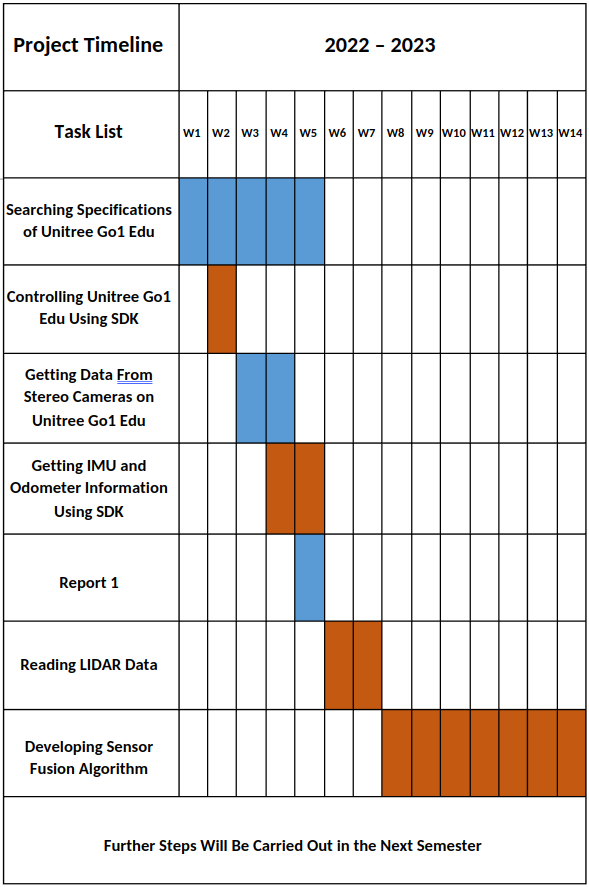
\includegraphics[width=0.65\textwidth]{GanttChart.png}
        \caption{Gantt Chart of Processes}
    \end{table}  

    
\section{ENGINEERING STANDARDS AND DESIGN \\ CONSTRAINTS}

The design constraints should be identified and some discussion on how these apply to the design project and their realization are to be included in this section. You may refer to the list of some realistic design constraints that can be found in the Project Design Constraints document. Other constraints can be identified and discussed, if applicable.  

    \subsection{ENGINEERING STANDARDS}
    
    We use the IEEE standards in our project. From the related pages~\cite{enwiki:1120084976} we found the good to have rules as follows:

    IEEE 829-2008, also known as the 829 Standard for Software and System Test Documentation, was an IEEE standard that specified the form of a set of documents for use in eight defined stages of software testing and system testing, each stage potentially producing its own separate type of document. The standard specified the format of these documents, but did not stipulate whether they must all be produced, nor did it include any criteria regarding adequate content for these documents. These were a matter of judgment outside the purview of the standard~\cite{enwiki:1105776890}. There will be a lot of test cases for the design. Since the system is complex, the test scenarios should be documented with known standard in order to maintenance independently from project contributors.

    A software requirements specification (SRS) is a description of a software system to be developed. It is modeled after business requirements specification (CONOPS). The software requirements specification lays out functional and non-functional requirements, and it may include a set of use cases that describe user interactions that the software must provide to the user for perfect interaction~\cite{enwiki:1117244157}. Since we have such a software system will be developed, it should lay on some standards to make the codes and all implementations reusable and modular.

    A software design description (a.k.a. software design document or SDD; just design document; also Software Design Specification) is a representation of a software design that is to be used for recording design information, addressing various design concerns, and communicating that information to the design’s stakeholders~\cite{enwiki:1105986397}. Similarly, the developed system should have standardized documentation as we said in earlier two standards. The three keywords for a good software design are: modular, reusable, and flexible.

    Of course, as the project progresses, it will be important that we comply with more detailed standards. We will continue to mention these in future reports.


    \subsection{DESIGN CONSTRAINTS}

    From the "Project Design Constraints" document, our constraints are:

    \begin{itemize}
        \item \textbf{Economy:} \\
        For the term project duration we have no spending other then the supervisors did. In case of further production, maintenance, we should spend around 18 dollars without counting the costs of the work put forward. We cannot find this such project on the market. But educational project like ours exist.
          
        \item \textbf{Environment:} \\
        Our robot is battery powered and now on it is only in the development process by different cases. Hence for now we do not have any power consumption calculations (also because we are focused on the software). The radiation we uncovered are on the ISM RF band, legally. And there is no serious pollution of noise, hopefully.

        \item \textbf{Manufacturability:} \\
        Physical implementation will consist of collecting materials and combining them due to use of ready made products. Since, there is no need for high level technologies of manufacturing.

        \item \textbf{Sustainability:} \\
        If we look at the reliability and durability of the design, we can say the legged robot that we use is waterproof but there are a few of external components those are not. Our project is a comprehensive study in which the mathematical foundations of a product that can serve humanity in many areas such as personal use, industrial use and use in disasters are laid and upper engineering problems are solved. In this way, its sustainability is high because it sits on a very comprehensive basis. Also upgrades for scaling purposes are possible to implement since the software we are developing has an abstraction from the hardware. 
        
    \end{itemize}

    and the other constraints for our project specifically due to usage of the some bought products are:

    \begin{itemize}
        \item \textbf{Computing Power}
            \begin{itemize}
                \item \textbf{Internal Nvidia Jetson Nano 4GB:} \\
                Mobile computing devices tend to have less computing power due to their size limits. There are three Nvidia Jetson Nano devices inside of the Unitree Go1 Edu. These devices located in the robot to perform certain tasks. Two of Nvidia Jetson Nano 4GB and one Nvidia Jetson Nano 2 GB development kits are used for getting data from camera and sensors, processing raw data to extract dept information of stereo cameras, human skeleton tracking and so on. 

                We don’t need most of the features of the robot like human tracking in our project, so we can lighten its workload and use one of them as our computing unit. 

                \item \textbf{External Nvidia Jetson:} \\
                In case of having a trouble with using internal Nvidia Jetson device, we can also use an external one. It can be again a Nvidia Jetson Nano with all resources dedicated to our sensor fusion algorithm or a more advanced model like Xavier Nx. This option will rise the cost of the project, so this is an option only if actually needed. 
            
                \item \textbf{Cloud Computing:} \\
                Computing is any goal-oriented activity requiring, benefiting from, or creating computing machinery~\cite{enwiki:1120224488}. There are different computing elements. CPU’s have ability to work high clock frequencies and have large set of sequential instructions. GPU’s are mostly  Mobile computing devices like Nvidia’s Jetson series development kits may not match the performance requirements in some cases. There are GPU servers to provide high parallel computing power.
                
            \end{itemize}

            \vspace{10pt}

            \begin{table}[H]
                \centering
                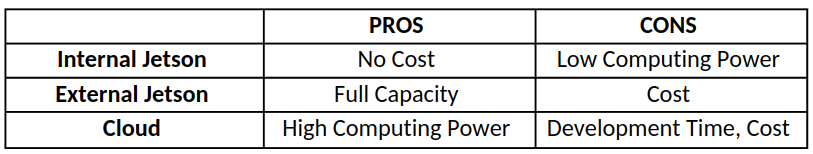
\includegraphics[width=0.8\textwidth]{ComputerComparison.png}
                \caption{Computing Power Comparison}
            \end{table}

            \textbf{Result:} 

            We decided to use Internal Jetson Development kits of the robot for sake of cost reduction. But as mentioned before, one of the aims of this project is moving execution of algorithms that need high computing power to the cloud. So, we will be using both internal Jetson devices and cloud computing. That will be give us an opportunity to compare results in both alternatives. 

        \item \textbf{Depth Sensor \& Stereo Camera}
            \begin{itemize}
                \item \textbf{Internal Unitree Camera – Super Sensory System:} \\
                Lens Angle ~150°×170° 

                \begin{figure}[H]
                    \centering
                    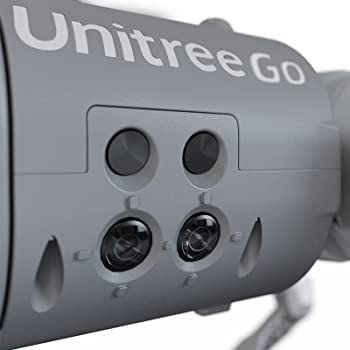
\includegraphics[width=0.5\textwidth]{SuperSensorySystem.png}
                    \caption{Super Sensory System}
                \end{figure}

                \item \textbf{External ZED Stereo Camera:} \\
                
                \begin{figure}[H]
                    \centering
                    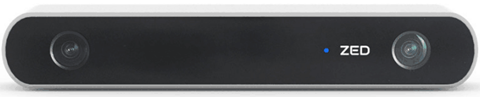
\includegraphics[width=0.5\textwidth]{ZEDCam.png}
                    \caption{ZED Stereo Camera~\cite{ZEDStereoCamera}}
                \end{figure}

                Some specifications of ZED: 

                \begin{itemize}
                    \item High-Resolution and High Frame-rate 3D Video Capture (1080p 30fps) 
                    \item Depth Perception indoors and outdoors at up to 20m 
                    \item 6-DoF Positional Tracking 
                    \item Spatial Mapping 
                    \item 110° Wide Angle Cameras 
                \end{itemize}

                \item \textbf{Xbox 360 Kinect:} \\
                \begin{figure}[H]
                    \centering
                    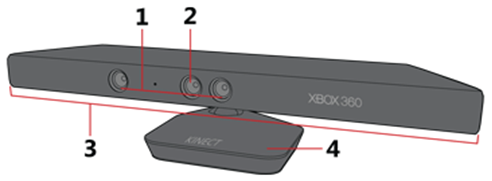
\includegraphics[width=0.5\textwidth]{XBoxKinect.png}
                    \caption{Xbox 360 Kinect~\cite{XboxKinect}}
                \end{figure}

                \begin{enumerate}
                    \item 3D Depth sensor (IR Emitter + IR Camera / Depth Sensor) 
                    \item RGB camera (Color Sensor) 
                    \item Microphone array 
                    \item Tilt motor (for detecting floor and players in the play space) 
                \end{enumerate}

                \item \textbf{Velodyne 80-VLP-16-A 3D LiDAR:} \\
                \begin{figure}[H]
                    \centering
                    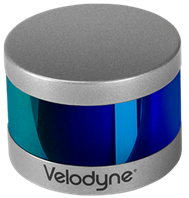
\includegraphics[width=0.3\textwidth]{LiDAR.png}
                    \caption{Velodyne LiDAR}
                \end{figure}

                Some specifications of LiDAR:

                \begin{itemize}
                    \item 100 m Range 
                    \item 360° x 30° Viewing Angle 
                    \item 0.3 Million Points/Second 
                    \item 100Mbps Ethernet \& UDP Interface 
                    \item Rated IP67 
                \end{itemize}
            \end{itemize}
        
        \vspace{10pt}

        \begin{table}[H]
            \centering
            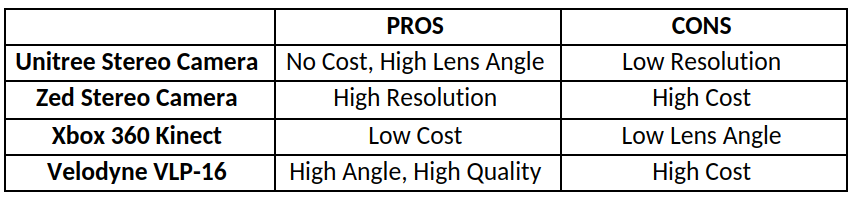
\includegraphics[width=0.8\textwidth]{SensorProsCons.png}
            \caption{Sensor Comparison}
        \end{table}

        \textbf{Result:} 

        As we consider the trade-offs that are given at table-x, we decided to move on with Unitree Stereo Cameras and Velodyne VLP-16 3D Lidar. 

        \item \textbf{Programming Languages} \\
        There are different tools we need to use to control the robot, access its sensor measurements and camera data etc. The robot manufacturer provides SDKs to access and control the robot. These SDKs are implemented using C++ programming language. 

        There is an SDK provided by Unitree to control robots with software. The SDK is implemented in C/C++ languages, but it supports programming in C, C++ and Python languages. So, at some point, we had to use those languages. 

        Besides these, ROS technology has a lot of programming languages provided. Since, we have no restriction from this side, hopefully. 

        \vspace{10pt}

        \textbf{Result:} 

        As we consider the performance and easy usage, we are planning to use Python only for algorithm development. After that we will be implement same algorithms in C++ to improve performance. SDK handles most of the ROS work, but we use ROS commands if it needed. 
        
    \end{itemize}


\section{SUSTAINABLE DEVELOPMENT GOALS}

Our project is a comprehensive study in which the mathematical foundations of a product that can serve humanity in many areas such as personal use, industrial use and use in disasters are laid and upper engineering problems are solved. In this way, its sustainability is high because it sits on a very comprehensive basis. If we look at our project in the context of global goals, it is a good example of Goal 9: Industry, Innovation, and Infrastructure. In addition, our design successfully complies with Goal 12: Responsible consumption and production, as abstractions are kept neatly. For example, scaling in design using the same software infrastructure is quite possible and simple.


\section{BACKGROUND}

For this project the need of strong background is irrefutable. Since there is software oriented design for our case, the reasearchs are more leading. Background comes from the earlier courses in our department, additional research, professional life, and even daily life. Also tricky parts are coming from experiences of our supervisors (know-hows, etc.).

    \subsection{BACKGROUND ACQUIRED IN EARLIER COURSE WORK}

    The sensor fusion operation require a lot mathematical theory and its practical implementations. At this point, the importance of our Calculus (MAT123/124) and Engineering Mathematics (MAT235/236), Signals and Systems (ELE301), Control Systems (ELE354), and Digital Signal Processing (ELE407) courses takes place. 

    But they are not enough to come up with a practical project. To design the system of this large computing environment and the network we should lay on the Computers and Programming (ELE107), Computer Programming (ELE118/120), Data Structures (ELE411), and Data Communication (ELE412) courses. For the sensor fusion operation we also use the knowledge from the Image Processing (ELE492) course for filtering bases and the hands-on programming purposes.

    \subsection{BACKGROUND ACQUIRED THROUGH ADDITIONAL\\ RESEARCH}

    Although our courses that we took in our department are pretty important for the theoretical base and introductory for the implementation, the know-hows of the programming languages, computer architectures, design patterns, and the protocols that we use are beyond from the course curriculums. To get those knowledge, we made a lot of research about those. Besides this, specifically the programming language practices are coming from our part-time jobs, internships, extracurricular studies, and further studies, and coding practices which coming from our supervisors suggestions.

    To be more specific, the CPP and the Python programming languages are not taught but we should already know those to go further in our design. Another example is ROS (robot operating system) concept that is special for our purposes has nothing to do with our courses. Sensor fusion is also a specific research area of the digital signal processing, control systems, mathematics, and Computer Vision~\cite{enwiki:1120271364} for ur case, obviously. Hence, we also made lots of preliminary study in this topic, other than courses.
    
\addcontentsline{toc}{section}{REFERENCES}
\bibliographystyle{plain}
\bibliography{refs}
\end{document}
